\documentclass[main.tex]{subfiles}

\begin{document}

\section{电影海报检索}

\subsection{应用场景}

本来我们想实现利用中文海报搜索对应电影信息的功能,但后来想到对于中国人来说,直接从海报中读出标题后在网上搜索更为方便快捷,不存在对于这个功能的需求,所以这个功能改为利用英文海报搜索对应的中文电影信息,受众是不太熟悉英文的人群。

\subsection{思路}

实现这个功能最关键的障碍在于我们无法使用各种快速哈希算法,因为我们希望这个功能的使用场景是用户利用摄像头拍摄海报照片上传至网页进行搜索,而大多数的图片哈希算法或者图片签名算法如 \cite{wong2002image} 要求被搜索图片在数据集中。同样,课程中讲到的 LSH 算法也不大满足我们的需求,因为因为用户上传的照片中有与海报无关的场景信息,这些场景信息对于 LSH 的计算来说是很大的干扰,所以最终决定利用 OCR 技术。

\subsection{实现}

以下为利用英文海报图片搜索电影信息的流程:

首先,我们利用 EAST 文本检测器 \cite{zhou2017east} 检测电影海报中的文字区域。比起直接对整张海报进行 OCR,先检测文字区域在对文字区域进行 OCR 的准确率更高,速度更快。EAST 检测文字的流程如下:

\begin{enumerate}
    \item 先用一个通用的网络(论文中采用的是 Pvanet,实际在使用的时候可以采用 VGG16,Resnet等)作为 base net,用于特征提取;
    \item 基于上述主干特征提取网络,抽取不同 level 的 feature map(它们的尺寸分别是 inuput-image 的 1/32,1/16,1/8,1/4),这样可以得到不同尺度的特征图。目的是解决文本行尺度变换剧烈的问题,early stage 可用于预测小的文本行,late stage 可用于预测大的文本行;
    \item 特征合并层,将抽取的特征进行 merge。这里合并的规则采用了 U-net 的方法,合并规则:从特征提取网络的顶部特征按照相应的规则向下进行合并,具体参见图~\ref{fig:east-net} 中的网络结构图;
    \item 网络输出层,包含文本得分和文本形状。根据不同文本形状可分为 RBOX 和 QUAD),输出也各不相同,具体参看图~\ref{fig:east-net}。
\end{enumerate}

\begin{figure}[h]
    \centering
    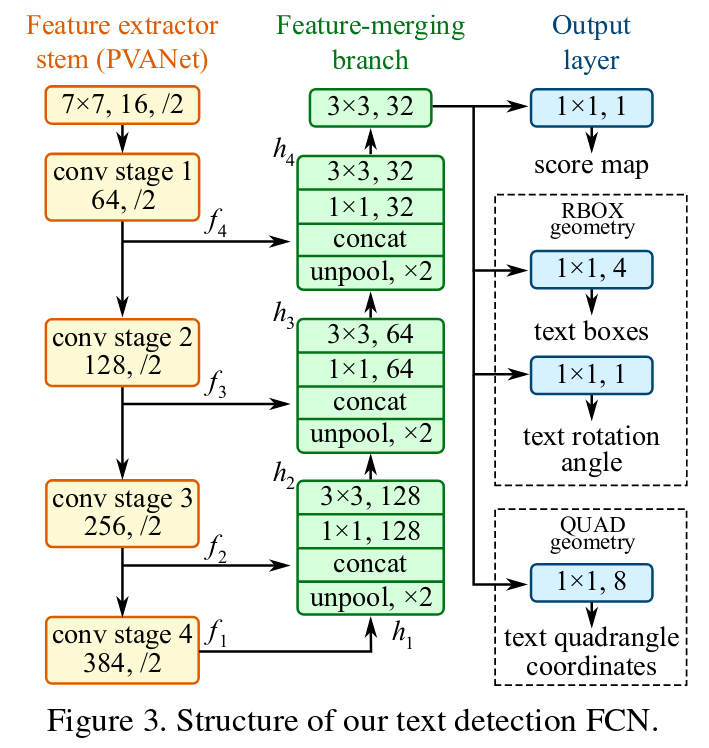
\includegraphics[width=0.5\linewidth]{images/east_net.png}
    \caption{EAST 文本检测网络结构图 \cite{zhou2017east}}
    \label{fig:east-net}
\end{figure}

EAST 的最大特点是能够检测倾斜的文字,所以下一步我们需要通过旋转矫正倾角较大的文字区域。然后,计算每一个文字区域的高度并按照文字高度排序,保留文字高度靠前的文字区域(我们的实现中选择的是文字高度前五的文字区域)。从原图中裁剪下这些文字区域进行 OCR。

OCR 方面我们利用的是 Google 的开源软件 Tesseract。Tesseract 的 OCR 模式选择单行文本识别和基于其内置神经网络的 OCR 算法。我们将每一个文字区域的文字识别结果收集起来进行文本搜索。

\subsection{评估}

图~\ref{fig:poster-good-for-ocr} 中给出了一些识别效果较好的电影海报,而图~\ref{fig:poster-bad-for-ocr} 中给出了一些具有代表性的识别效果较差的海报。从这些海报中我们大致可以总结出识别效果差的原因:

\begin{enumerate}
    \item 识别效果差很大程度上是 OCR 的原因而不是文字检测的原因;
    \item OCR 提高准确率的关键在于字体训练,而海报标题中有很多风格迥异的花体或艺术体的字母,Tesseract 就无法识别。例如,图~\ref{fig:poster-bad-for-ocr} 中的第一张和第三章海报无法识别出标题很可能仅仅是因为海报标题的字体中笔画之间有间隙。
\end{enumerate}

\begin{figure}
    \centering
    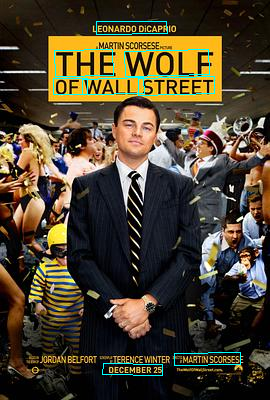
\includegraphics[width=0.3\linewidth]{images/poster_good_1.png}
    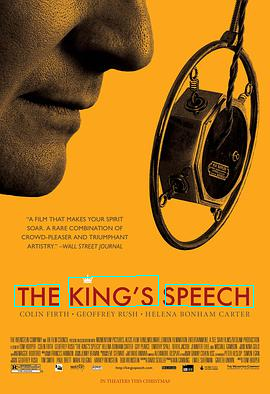
\includegraphics[width=0.3\linewidth]{images/poster_good_2.png}
    
\includegraphics[width=0.3\linewidth]{images/poster_good_3.png}
    \caption{识别效果好的电影海报(淡蓝色框为文字区域)}
    \label{fig:poster-good-for-ocr}
\end{figure}

\begin{figure}
    \centering
    
\includegraphics[width=0.3\linewidth]{images/poster_bad_1.png}
    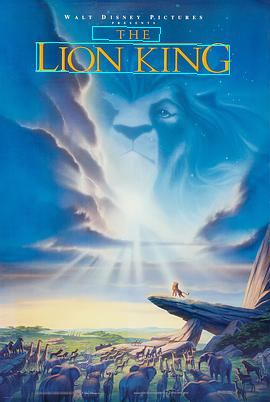
\includegraphics[width=0.3\linewidth]{images/poster_bad_2.png}
    
\includegraphics[width=0.3\linewidth]{images/poster_bad_3.png}
    \caption{识别效果差的电影海报(淡蓝色框为文字区域)}
    \label{fig:poster-bad-for-ocr}
\end{figure}

\subsection{改进}

Huang 等人提出 \cite{huang2015text} 在英文海报提取标题时可以利用拼写检查功能修正常见的 OCR 错误。

\section{电影搜索}

\subsection{应用场景}

当用户走在街上时,被屏幕中有关最新上映电影的预告片所吸引,而又不想停下脚步等待预告片播完时最终出现的电影名字,就可以拍下预告片并上传到我们的系统进行搜索来获取电影信息。

\subsection{思路}

我们将预告片转换为一系列的帧来进行图像处理,而这样会导致数据集中的图片数量过于巨大,而我们又希望能够在合理的时间内返回结果,所以最终采用的仍然是图片搜索转换成文字搜索的这一主要思路。首先是识别预告片中的字幕,然后利用字幕进行文字搜索,寻找对应的电影。

\subsection{实现}

从预告片视频文件中读取每一帧,然后对每一帧做一系列预处理以提高 OCR 精确度。例如,字幕一般位于视频中偏下的位置,所以预处理包含了裁剪这一步骤。又因为大部分的字幕都是白色,裁剪完的图片先转换成灰度图片,再二值化。图~\ref{fig:frame-preprocessing} 中给出了图片预处理前后的对比。

\begin{figure}[h]
    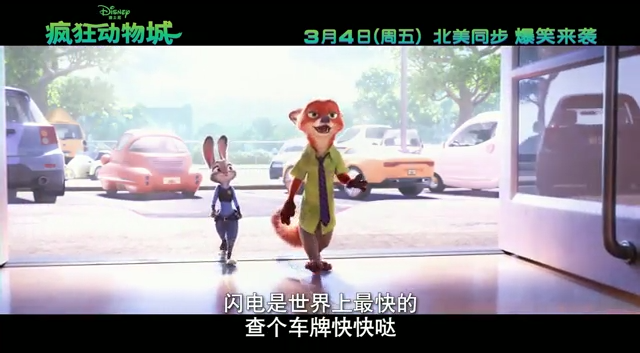
\includegraphics[width=0.5\linewidth]{images/frame_before_preprocessing.png}
    
\includegraphics[width=0.5\linewidth]{images/frame_after_preprocessing.png}
    \caption{帧的预处理(左图为直接从预告片中提取的原始帧,右图为预处理的输出图片)}    \label{fig:frame-preprocessing}
\end{figure}

在 OCR 方面,我们先尝试了使用 Tesseract 内置的中文文字识别,发现结果难以接受,识别的准确率基本是零,似乎 Tesseract 只能识别最简单的中文字符。接下来我们又尝试了 CTPN \cite{tian2016detecting} 用于文字检测和 CRNN 用于文字识别。CTPN 文字检测的流程(参见图~\ref{fig:ctpn-pipeline})如下:

\begin{figure}[h]
    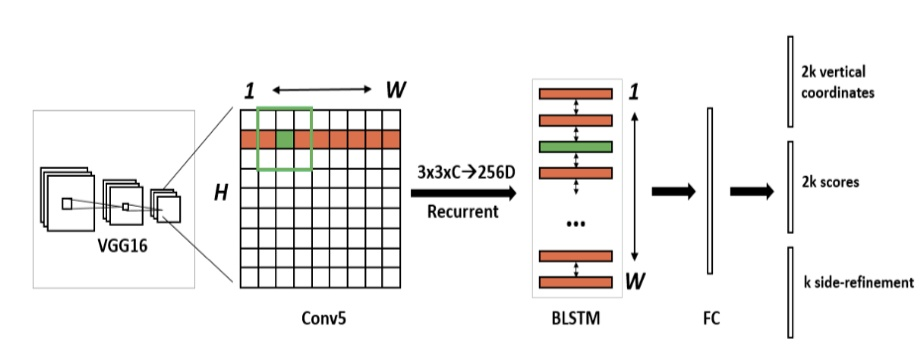
\includegraphics[width=\linewidth]{images/ctpn_pipeline.jpg}
    \caption{CTPN 文字检测流程图 \cite{tian2016detecting}}
    \label{fig:ctpn-pipeline}
\end{figure}

\begin{enumerate}
    \item 首先,用 VGG16 的前 5 个 Conv stage 得到 feature map,大小为 $W \times H \times C$
    \item 用 $3 \times 3$ 的滑动窗口在前一步得到的 feature map 上提取特征,利用这些特征来对多个 anchor 进行预测,这里 anchor 定义与之前 faster-rcnn 中的定义相同,也就是帮我们去界定出目标待选区域。
    \item 将上一步得到的特征输入到一个双向的 LSTM 中,输出 W*256 的结果,再将这个结果输入到一个 512 维的全连接层(FC).
    \item 最后通过分类或回归得到的输出主要分为三部分,根据上图从上到下依次为 2k vertical coordinates,表示选择框的高度和中心的 y 轴的坐标;2k scores 表示的是 k 个 anchor 的类别信息,说明其是否为字符;k side-refinement 表示的是选择框的水平偏移量。本文实验中 anchor 的水平宽度都是 16 个像素不变,也就是说我们微分的最小选择框的单位是 16 像素。    
    \item 用文本构造的算法,将我们得到的细长的矩形合并成文本的序列框。
\end{enumerate}

事实上,我们演示时用的就是这一技术组合,但在最终整合时发现 CTPN 仅仅在几部预告片中有着较好的效果,将其广泛应用到其他预告片时效果并不好。由于时间原因,我们最后选择的是 Yolo 3 + CRNN 的开源 OCR 实现 chineseocr。

以上介绍的是 OCR 技术。这个功能还有一个实现难点是,搜索时我们利用某一帧中的字幕放入 Elasticsearch 进行文字搜索,而我们没有文本格式的预告片字幕来建立 Elasticsearch 的索引。所以我们先处理所有预告片,利用上文提到的 OCR 技术构建字幕文件。下面是给出重构完的字幕文件(只有部分):

\begin{verbatim}
    11.24 我要查个车牌号
    11.28 我要查个车牌号
    11.32 我要查个车牌号
    11.36 我要查个车牌号
    11.4 我要查个车牌号
    11.44 我要查个车牌号
    11.48 我要查个车牌号
    11.52 我要查个车牌号
    11.56 我要查个车牌号
\end{verbatim}

字幕文件中是每一行字幕及其对应的视频中的时间。利用这个便可以建立索引。

\subsection{评估}

由于构造用于对比的 ground truth 非常困难(上面已经提到,我们没有预告片原始的字幕文件),这里的准确率是估计的结果。chineseocr 在我们的应用场景中能够有着高达 90\% 的准确率,绝大部分的文字都能够准确识别,我们认为这是因为 chineseocr 训练用的中文字体和常见的用于制作字幕的字体非常相似。

\subsection{改进}

利用字幕进行电影搜索有两个显而易见的缺陷:

\begin{enumerate}
    \item 一行字幕在预告片中会停留一段时间,即一段字幕会对应多个帧;
    \item 无法搜索没有字幕的帧。
\end{enumerate}

第一个缺陷这样改进:先利用字幕缩小搜索范围到具体的某几帧,再利用图像特征匹配(如 SIFT)进行精确匹配。第二个缺陷是我们这种搜索方法无法回避的,但为了能够提供足够的搜索速度,我们还是采用了字幕搜索而放弃了功能。

\end{document}
